\documentclass[a4paper,12pt]{article}
\usepackage[indonesian]{babel}
\usepackage{graphicx}
\usepackage{multirow}
\usepackage{enumitem}
\usepackage{listings}
\usepackage{wrapfig}
\usepackage[T1]{fontenc}
\usepackage{inconsolata}
\usepackage{lipsum}
\usepackage{adjustbox}


\usepackage{color}
\usepackage[table]{xcolor}
\definecolor{mygreen}{rgb}{0,0.6,0}
\definecolor{mygray}{rgb}{0.5,0.5,0.5}
\definecolor{mymauve}{rgb}{0.58,0,0.82}
\lstset{%
    language=java,
    showstringspaces=false,          % Prevent tex replacing space to bracket in code
    frame=single,                    % Set frame around code
    backgroundcolor=\color{white},   % choose the background color
    basicstyle=\footnotesize,        % size of fonts used for the code
    breaklines=true,                 % automatic line breaking only at whitespace
    captionpos=b,                    % sets the caption-position to bottom
    commentstyle=\color{mygreen},    % comment style
    keywordstyle=\color{blue},       % keyword style
    stringstyle=\color{mymauve},     % string literal style
    numbers=left,
}

\graphicspath{ {./img/} }
\begin{document}
\title{ {\Large Laporan Praktikum}\\ Algoritma dan Pemrograman Lanjut\\{\Large Pertemuan 12}}

\author{Aldzikri Dwijayanto Prathama
    \\195410189
    \\Informatika}
\makeatletter
\begin{titlepage}
    \begin{center}
        {\huge \bfseries \@title}\\[14ex]
        
\includegraphics[scale=.8]{logo}\\[4ex]
        {\large \@author}\\[12ex]
        {\large \bfseries {SEKOLAH TINGGI MANAJEMEN INFORMATIKA DAN KOMPUTER
            AKAKOM YOGYAKARTA}}
    \end{center}


%{\large \@date}
\end{titlepage}
\makeatother
%\maketitle
\newpage
\tableofcontents
\newpage

\section{Tujuan}
Mahasiswa dapat  memahami dan membedakan rekursif dan iterasi serta mengubah rekursif menjadi iterasi.
\section{Teori}
Iterasi menggunakan pernyataan pengulangan, sedangkan rekursi menggunakan
pernyataan seleksi. Baik iterasi dan rekursi melibatkan pengulangan: Iterasi secara eksplisit
menggunakan pernyataan pengulangan, sedangkan rekursi mencapai pengulangan melalui pemanggilan method berulang. Iterasi
dan rekursi masing-masing melibatkan tes terminasi: Iterasi berakhir ketika kondisi loop bernilai false sedangkan
rekursi berakhir ketika case dasar tercapai.\\

Iterasi dengan pengulangan dan rekursi yang dikontrol secara bertahap mendekati penghentian: Iterasi terus memodifikasi
penghitung hingga penghitung mengasumsikan nilai yang membuat kondisi loop bernilai false, sedangkan rekursi terus
menghasilkan versi yang lebih kecil dari masalah awal hingga case dasar tercapai. Baik iterasi dan rekursi dapat terjadi
hingga tak terhingga: Loop tak terbatas terjadi dengan iterasi jika uji kelanjutan loop tidak pernah menjadi salah,
sedangkan rekursi tak terbatas terjadi jika langkah rekursi tidak mengurangi masalah setiap kali dengan cara yang
menyatu pada case dasar, atau jika case dasar tidak diuji.

\newpage

\section{Pembahasan}
\subsection{Praktik}
\subsubsection{Praktik 1}
\begin{lstlisting}
public class FaktorialIterasi {
    public static void main(String[] args) {
        int batas = 5;
        int counter = 0;
        int faktorial = 1;
        for (counter = 1; counter <= batas; counter++)
            faktorial *= counter;
        System.out.println("Nilai " + batas + "!" + " adalah " + faktorial);
    }
}
\end{lstlisting}

Pada program praktik pertama adalah membuat untuk menghitung faktorial dengan menggunakan iterasi. Untuk menghitung
faktorila tersebut digunakan looping for, yang didalamnya terdapat pernyataan untuk mengalikan faktorial dengan counter,
dan memasukan hasilnya kembali ke variabel faktorial.

\begin{center}
    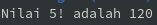
\includegraphics[scale=1]{1.png} 
\end{center}

\subsubsection{Praktik 2}
\begin{lstlisting}
public class FibonacciIterasi {
    public static void main(String[] args) {
        System.out.println("Deret fibonacci dengan N = 5");
        int fibn;
        int fibn1 = 1;
        int fibn2 = 0;
        for (int i = 0; i <= 5; i++)
            if (i == 0 || i == 1)
                System.out.print(i + " ");
            else {
                fibn = fibn1 + fibn2;
                fibn2 = fibn1;
                fibn1 = fibn;
                System.out.print(fibn + " ");
            }
    }
}
\end{lstlisting}
Pada praktik 2 ini kita akan mebuat program untuk menghitung Fibonacci dengan iterasi. Bisa dilihat pada gambar program dibawah, pada
baris ke-4 kita tambahkan variabel fibn, pada baris ke-5 kita tambahkan variabel fibn1 dengan valuenya 1 dan pada baris
ke-6 kita tambahkan variabel fibn2 dengan valuenya 0, ketiga variabel tersebut memiliki tipe data integer. Kemudian pada
baris ke-7 kita tambahkan perulangan for yang didalamnya (baris ke-8 sampai 14) kita tambahkan seleksi if.

\begin{center}
    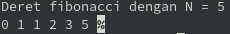
\includegraphics[scale=1]{2.png} 
\end{center}


\subsubsection{Praktik 3}
\begin{lstlisting}
package praktik12;

/**
 * FaktorialRekursif
 */
public class FaktorialRekursifIterasi {

    public static long faktorial(long N) {
        long bil = N;
        if (N <= 1) {
            bil = 1;
        }
        else {
            long tmp = N-1;
            System.out.print(bil + ", ");
            for(long i = N; i > 1; i--) {
                bil = bil * tmp;
                tmp -= 1;
                System.out.print(bil + ", ");
            }
                
        }
        return bil;
    }

    public static void main(String[] args) {
        System.out.println("Faktorial 5 = " + faktorial(5));
    }
}
\end{lstlisting}
Tugas untuk Praktik 3, adalah mengubah program praktik 3 pada pertemuan 11 dari rekursif menjadi iterasi. Pad method
faktorial, terdapat seleksi if, dan didalam else, terdapat perulangan for yang akan menghitung faktorial dengan
menggunakan iterasi

\begin{center}
    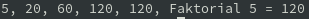
\includegraphics[scale=1]{3.png} 
\end{center}

\newpage

\subsection{Latihan}
\subsubsection{Latihan 1}

Untuk tugas latihan pertama adalah membuat program untuk mengeprint elemen array menggunakan rekursif dan iterasi.

\textbf{Rekursif\\}
\begin{lstlisting}
package praktik12;

/**
 * PrintElemenRekursif
 */
public class PrintElemenRekursif {

    private static int printArray(int[] N,int A) {
        if(A == N.length){
            return 0;
        } else {
            System.out.print(N[A] + " ");
            return printArray(N, A+1);
        }
    }

    public static void main(String[] args) {
        int[] bil = {1,2,3,4,5,6};
        int hit = 0;
        printArray(bil,hit);
        System.out.println();
    }
}
\end{lstlisting}
Untuk rekursif, dibuat dua method, metho pertama berfungsi untuk mengeprint, di dalamnya terdapat seleksi if, yang jika
nilai A sudah sebanding dengan panjang data N, maka program akan mengembalikan nilai 0, dan berhenti. Pada else terdapat
pernyataan untk mengeprint elemen, dan pernyataan rekursif.
\begin{center}
    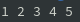
\includegraphics[scale=1]{4.png} 
\end{center}

\textbf{Iterasi\\}
\begin{lstlisting}
package praktik12;

/**
 * PrintElemenIterasi
 */
public class PrintElemenIterasi {

    private static void printArray(int[] N) {
        int[] bil = N;
        for (int i = 0; i < bil.length; i++) {
           System.out.print(bil[i] + " ");
        }
    }

    public static void main(String[] args) {
        int[] bil = {1,2,3,4,5};
        printArray(bil);
        System.out.println();
    }
}
\end{lstlisting}
Untuk iterasi juga dibuat dua method. Method pertama memiliki perulangan for, yang didalamnya terdapat pernyataan untuk
mengeprint elemen dalam array. Kemudian method main berguna untuk memasukkan nilai, dan memanggil method pertama.
\begin{center}
    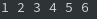
\includegraphics[scale=1]{5.png} 
\end{center}

\subsubsection{Latihan 2}

Tugas latihan 2 adalah membuat program yang akan membalik string yang dimasukkan menggunakan rekursif dan iterasi.\\

\textbf{Rekursif\\}
\begin{lstlisting}
package praktik12;

public class CharArrayRec {
    public static void stringReverse(char[] array, int index) {
        if (index > -1) {
            System.out.print(array[index]);
            stringReverse(array, index - 1);
        }
    }

    public static void stringReverse(String kata) {
        char[] array = kata.toCharArray();
        stringReverse(array, array.length - 1);
    }

    public static void main(String args[]) {
        String kata = "Contoh kata yang akan di balik";
        stringReverse(kata);
    }
}
\end{lstlisting}

Pada baris ke-2 kita tambahkan array bertipe data char dan variabel index dengan tipe data integer. Pada baris ke-3 kita
tambahkan seleksi if dengan kondisi index lebih dari -1. Pada baris ke-4 kita tambahkan perintah untuk menampilkan
array. Kemudian pada baris berikutnya kita tambahkan method stringReverse dengan didalamnya array dan index-1.
Selanjutnya pada baris ke-10 kita tambahkan array dengan valuenya kata.toCharArray, Method ini mengalokasikan array
karakter baru, yang panjangnya sesuai dengan panjang string yang ditentukan dan isinya diinisialisasi mengandung urutan
karakter diwakili oleh string yang ditentukan.

\begin{center}
    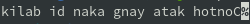
\includegraphics[scale=1]{6.png} 
\end{center}

\textbf{Iterasi\\}
\begin{lstlisting}
package praktik12;

public class CharArrayIte {
    public static void main(String args[]) {
        String kata = "Contoh kata yang akan di balik";
        char[] array = kata.toCharArray();
        int index = array.length - 1;
        while (true) {
            if (index > -1) {
                System.out.print(array[index]);
                index--;
            } else {
                break;
            }
        }
    }
}
\end{lstlisting}
Pada baris ke-3 kita tambahkan variabel kata dengan tipe data integer. Kemudian pada baris ke-4 kita tambahkan array dengan value kata.toCharArray. Pada baris ke-5 kita tambahkan variabel index dengan value panjang array – 1. Pada baris ke-6 kita tambahkan perulangan while dengan kondisi true didalamnya kita tambahkan seleksi if.
\begin{center}
    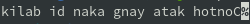
\includegraphics[scale=1]{6.png} 
\end{center}

\subsubsection{Latihan 3}

Untuk latihan 3 adalah membuat program untuk mencari nilai terkecil pada array menggunakan rekursif dan iterasi.\\

\textbf{Rekursif}
\begin{lstlisting}
package praktik12;

/**
 * ElemenTerkecil
 */
public class ElemenTerkecil {
    public static int recursiveMinimum(int[] angka, int index) {
        int kembalian = angka[0];
        if (index < angka.length) {
            kembalian = recursiveMinimum(angka, index + 1);
            int terendah = angka[index];
            if (terendah < kembalian) {
                kembalian = terendah;
            }
        }
        return kembalian;
    }

    public static void main(String args[]) {
        int[] angka = { 68, 43, 53, 52, 74, 24, 46 };
        System.out.println("Angka terkecil dari array:" +

                recursiveMinimum(angka, 0));
    }
}

\end{lstlisting}
Pada baris ke-2 kita tambahkan array angka dan variabel index. Pada baris ke-3 kita tambahkan variabel kembalian dengan value angka array 0. Kemudian pada baris ke-4 kita tambahkan seleksi if. Pada baris ke-16 kita tambahkan perintah untuk menampilkan outputnya.
\begin{center}
    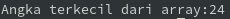
\includegraphics[scale=1]{7.png} 
\end{center}

\textbf{Iterasi}
\begin{lstlisting}
package praktik12;

/**
 * ElemenTerkecilIterasi
 */
public class ElemenTerkecilIterasi {

    public static void main(String[] args) {
        int[] bil = {3,4,1,2,8,9,2,0};
        int hasil = bil[0];
        for(int i = 0; i < bil.length; i++) {
            if(hasil > bil[i]) {
                hasil = bil[i];
            }
        }
        System.out.println(hasil);
    }
}
\end{lstlisting}
Untuk iterasi, pada perulangan for terdapat pernyataan yang akan membandingkan nilai dari array, jika nilai lebih kecil
dari nilai pada variabel hasil, maka nilai dari variabel hasil tersebut akan diganti dengan bilangan yg lebih kecil
tadi.
\begin{center}
    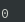
\includegraphics[scale=1]{8.png} 
\end{center}


\newpage

\subsection{Tugas}
\subsubsection{Tugas 1}
Untuk tugas pertama adalah menbuat program untuk menghitung pangkat menggunakan iterasi.

\begin{lstlisting}
package praktik12;

import java.util.Scanner;

/**
 * PangkatIterasi
 */
public class PangkatIterasi {

    private static double hitungPangkat(double A, double B){
        double hasil = A;
        for(int i=1; i<B; i++){
            hasil = hasil * A;
        }
        return hasil;
    }

    public static void main(String[] args){
        Scanner in = new Scanner(System.in);
        double A = in.nextDouble();
        double B = in.nextDouble();
        in.close();
        System.out.printf("Hasil dari %.1f pangkat %.1f adalah %.1f \n", A, B, hitungPangkat(A,B));
    }
}
\end{lstlisting}
Pada program tersebut, terdapat dua method. Method pertama terdapat perulangan yang akan mengalikan variabel hasil, yang
sudah diberi nilai sama dengan A, dengan variabel A, dan menyimpan hasilnya ke variabel hasi. Method kedua, yaitu method
main berfungsi untuk memasukkan nilai, dan memanggil method pertama.
\begin{center}
    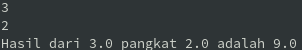
\includegraphics[scale=1]{9.png} 
\end{center}

\subsubsection{Tugas 2}
Tugas kedua adalah membuat program untuk mengecek apakah sebuah string palindrom atau bukan, menggunakan iterasi.
\begin{lstlisting}
package praktik12;

import java.util.Scanner;

/**
 * PalindromeIterative
 */
public class PalindromeIterative {

    private static boolean palCheck(String Pal){
        int a=0;
        int b=Pal.length()-1;
        while(b > a) {
            char depan = Pal.charAt(a);
            char belakang = Pal.charAt(b);
            if(depan != belakang){
                return false;
            }
            a++;
            b--;
        }
        return true;
    }

    public static void main(String[] args){
        Scanner in = new Scanner(System.in);
        String kata = in.nextLine();
        in.close();
        if(palCheck(kata)){
            System.out.printf("kata %s adalah palindrome \n", kata);
        }else{
            System.out.printf("kata %s bukan palindrome \n", kata);
        }
    }
}
\end{lstlisting}
Pada method pertama terdapat perulangan whilem yang di dalamnya terdapat pernyataan untuk membandingkan antara karakter
bagian depan dan akhir string, jika karakter tidak sama, maka method akan mengembalikan value false, jika semua karakter
sama, maka method akan mengembalikan value true.
\begin{center}
    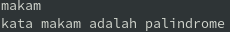
\includegraphics[scale=1]{10.png} 
\end{center}

\newpage

\section{Kesimpulan}
Setelah praktik mahasiswa paham dan mampu membedakan rekursif dan iterasi serta mengubah rekursif menjadi iterasi.
\end{document}
